\section{方法验证}
\label{sec:method_validation}

前述小节从方法角度说明了 PlanGraph 如何通过任务结构化、规划生成、知识检索、程序执行和反馈修复降低图推理错误。为了验证上述机制是否真正改善求解质量，实验分析围绕两个问题展开：第一，规划反馈式方法是否能够在不同图推理任务上带来稳定收益；第二，这种收益主要出现在哪些任务类型和错误场景中。相关结果主要刻画规划、检索和执行验证闭环对任务求解质量的影响。

\subsection{方法验证目标与数据集}

本文选取五个图推理基准测试集进行方法验证，包括 GraphArena\cite{tang2025grapharena}、NLGraph\cite{chen2024nlgraph}和 GraphWiz\cite{gong2024graphwiz}，以及 LLM4DyG\cite{llm4dyg2024}和 GraphInstruct\cite{graphinstruct2024}。这些数据集共同覆盖经典图算法、组合优化、自然语言图任务、动态图查询和指令式图操作等场景，既包含以节点、边和权重为核心输入的抽象图推理问题，也包含以自然语言场景或指令形式描述的实际场景化图推理问题。

对比方法包括 GPT-4o\cite{openai2024gpt4o}直接推理、多智能体图推理方法 GraphTeam\cite{li2024graphteam}以及程序生成式图推理方法 GCoder\cite{zhang2025gcoder}。三者分别代表直接提示推理、多智能体协同和程序生成求解路线，用于比较规划反馈闭环相对于现有图推理方法的效果。

从去除数据集内部重复任务后的任务类别看，GraphArena 包含 10 类任务，NLGraph 包含 8 类任务，GraphWiz 包含 9 类任务，LLM4DyG 包含 9 类任务，GraphInstruct 包含 21 类任务。本文在保持公开任务定义不变的前提下统一评价口径，主实验采用精确匹配率（Exact Match, EM）作为评价指标。任务类别和逐任务结果能够反映规划反馈机制在不同图推理场景中的具体作用。

\subsection{不同任务类别上的方法效果}

为了分析规划反馈机制在哪些任务上发挥作用，本文将多个基准测试集中的任务按照求解目标划分为图结构分析、最短路径、匹配问题、流优化和哈密顿类问题五个类别，并统计不同方法在各类任务上的平均表现，如图\ref{fig:category_accuracy_comparison}所示。

\begin{figure}[htbp]
\centering
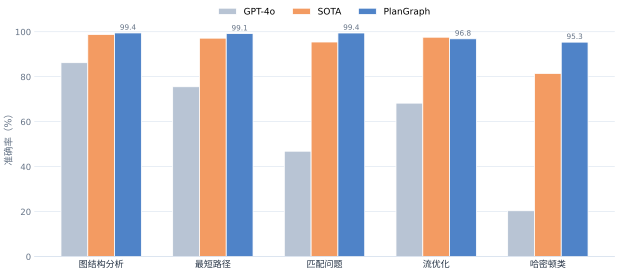
\includegraphics[width=0.94\textwidth]{figures/paper/exp_category_accuracy.pdf}
\caption{不同任务类别上的精确匹配率对比}
\label{fig:category_accuracy_comparison}
\end{figure}

由图\ref{fig:category_accuracy_comparison}可以看出，PlanGraph 在图结构分析、最短路径、匹配问题、流优化和哈密顿类五类任务上均取得了最高精确匹配率。其中，哈密顿类任务的提升幅度最明显。PlanGraph 的平均精确匹配率为 95.33\%，相比最佳现有方法的 74.30\% 高出 21.03 个百分点。该类任务通常同时涉及节点不重复访问、相邻节点连通、回路闭合以及总代价优化等要求。若直接由模型生成答案，容易出现节点遗漏、节点重复访问、路径不可行或代价计算错误等问题。PlanGraph 通过显式规划、程序执行和结果验证，将这些约束转化为可检查的步骤，因此能够更好地减少端到端生成中的结构性错误。

在流优化任务上，PlanGraph 也优于最佳现有方法。具体而言，PlanGraph 在 NLGraph-MF 和 GraphWiz-MF 两个最大流任务中均取得最优结果，两项任务的平均精确匹配率为 96.32\%，相比最佳现有方法的平均结果 94.40\% 提升 1.92 个百分点。最大流任务通常涉及残量图维护、容量更新、反向边处理和增广路径选择等实现细节，对程序实现和 API 使用都有较高要求。PlanGraph 在该类任务上的优势表明，规划生成和外部图算法知识检索能够帮助系统减少最大流求解中的实现偏差。

\subsection{复杂度与样本难度分层分析}

为考察 PlanGraph 在不同计算复杂度任务上的表现，本文将任务划分为 NP 完全任务与非 NP 完全任务两类。按照任务集合中的公开任务定义，本文将邻居查询、距离计算、连通分量和图直径等基础图任务划为非 NP 完全组，将最大独立集、最小点覆盖、最大团、图编辑距离、最大公共子图和旅行商问题划为 NP 完全组。图\ref{fig:np_complete_performance}展示了两类任务上的性能对比。

\begin{figure}[htbp]
\centering
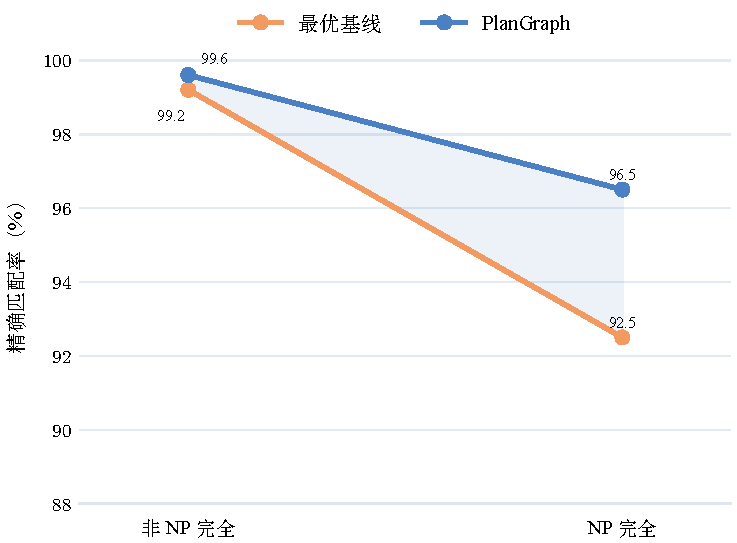
\includegraphics[width=0.86\textwidth]{figures/paper/exp_complexity_trend.pdf}
\caption{NP 完全任务性能对比}
\label{fig:np_complete_performance}
\end{figure}

可以看到，PlanGraph 在非 NP 完全任务上与最佳基线方法均达到 100.00\%，说明基础图任务已经接近饱和，提升空间有限；而在 NP 完全任务上，PlanGraph 的平均精确匹配率达到 96.23\%，较最佳基线方法的 92.87\% 提升 3.36 个百分点，说明规划与验证闭环的主要收益集中体现在高组合复杂度场景。这与最大独立集、最小点覆盖、最大团、图编辑距离、最大公共子图和旅行商问题等任务上的观察一致。

除任务复杂度外，本文还从样本难度角度观察方法表现。该划分以图规模为主要依据：简单样本对应节点数小于 15 的图实例，中等样本对应节点数为 15 至 30 的图实例，困难样本对应节点数大于 30 的图实例。图\ref{fig:sample_difficulty_performance}给出了不同难度样本上的性能对比。

\begin{figure}[htbp]
\centering
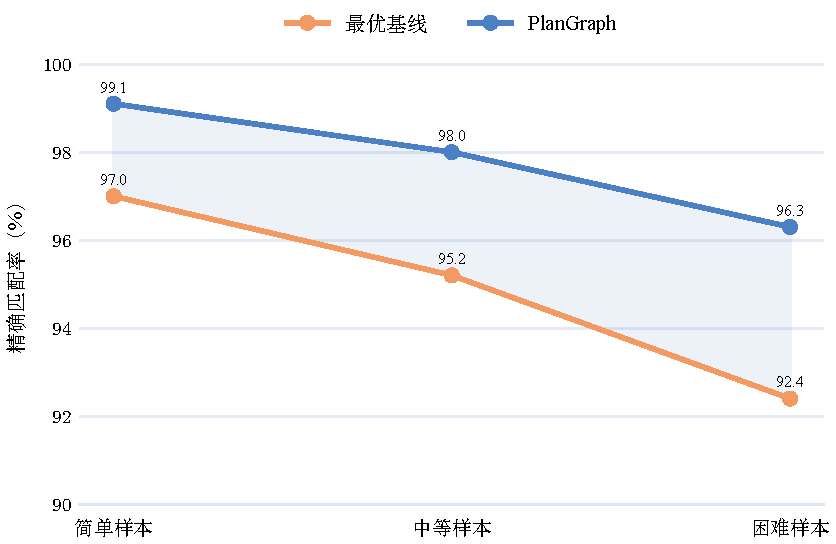
\includegraphics[width=0.86\textwidth]{figures/paper/exp_sample_difficulty_trend.pdf}
\caption{样本难度分层下性能对比}
\label{fig:sample_difficulty_performance}
\end{figure}

从图\ref{fig:sample_difficulty_performance}可见，随着样本难度提高，不同方法的性能均出现下降，但 PlanGraph 的下降幅度相对更小。尤其在困难样本上，PlanGraph 相比最佳基线方法的优势进一步扩大，说明规划先行与执行验证机制对大搜索空间下的稳定求解具有更明显作用。综合两类分层结果可以看出，PlanGraph 的性能收益主要来源于复杂任务场景，而非简单任务上的边际提升。

\subsection{各基准测试集逐任务结果}

为避免总体平均结果掩盖不同任务族之间的性能差异，本文进一步给出五个基准测试集的逐任务精确匹配率统计，以从更细粒度上分析 PlanGraph 在不同图推理场景中的适用性与性能边界。

GraphArena\cite{tang2025grapharena}是面向图计算与图推理任务的综合基准测试集，覆盖邻居查询、连通分量、最短距离、图直径、图编辑距离以及多类组合优化问题。表\ref{tab:grapharena_detail}给出了各方法在该基准测试集各子任务上的逐项结果。其中，CN、CC、SD、GD 和 GED 分别表示邻居查询、连通分量、最短距离、图直径和图编辑距离任务；MIS、MVC、MCP、MCS 和 TSP 分别表示最大独立集、最小点覆盖、最大团、最大公共子图和旅行商问题。

\begin{table}[htbp]
\centering
\caption{GraphArena 各任务精确匹配率（\%）}
\label{tab:grapharena_detail}
\begin{tabular}{lcccc}
\toprule
任务 & GPT-4o & GraphTeam & GCoder & PlanGraph \\
\midrule
CN & \textbf{100.0} & \textbf{100.0} & \textbf{100.0} & \textbf{100.0} \\
CC & \textbf{100.0} & \textbf{100.0} & \textbf{100.0} & \textbf{100.0} \\
SD & \textbf{100.0} & \textbf{100.0} & \textbf{100.0} & \textbf{100.0} \\
GD & \textbf{100.0} & \textbf{100.0} & \textbf{100.0} & \textbf{100.0} \\
GED & 23.3 & 91.0 & 89.5 & \textbf{96.5} \\
MIS & 22.4 & 97.8 & 96.8 & \textbf{98.8} \\
MVC & 19.3 & 98.6 & 97.6 & \textbf{100.0} \\
MCP & 12.5 & 90.5 & 88.7 & \textbf{100.0} \\
MCS & 8.4 & 90.8 & 89.4 & \textbf{95.3} \\
TSP & 4.9 & 82.7 & 80.7 & \textbf{86.8} \\
\bottomrule
\end{tabular}
\end{table}

表\ref{tab:grapharena_detail}显示，基础结构任务对各强基线均已较为简单，CN、CC、SD 和 GD 等子任务几乎都达到满分；图编辑距离和组合优化任务则具有较强区分度。PlanGraph 在这些高约束任务上保持更优结果，说明规划生成、知识检索和执行验证的闭环机制并非只在基础任务的饱和区间内带来边际改善，而是能够更有效地提升复杂图搜索任务中的可行性控制与错误修复能力。

NLGraph\cite{chen2024nlgraph}主要考察自然语言条件下的图算法推理能力，其核心难点不只在于调用某个图算法，而在于先从自然语言描述中恢复图结构、任务目标和求解约束，再完成相应的算法推理。表\ref{tab:nlgraph_detail}给出了各方法在 NLGraph 各子任务上的逐项结果。其中，CONN、MF、CYC、TOPO、SP、BM、HP 和 GNN 分别表示连通性、最大流、环检测、拓扑排序、最短路径、二分图匹配、哈密顿路径和 GNN 推理任务。

\begin{table}[htbp]
\centering
\caption{NLGraph 各任务精确匹配率（\%）}
\label{tab:nlgraph_detail}
\begin{tabular}{lcccc}
\toprule
任务 & GPT-4o & GraphTeam & GCoder & PlanGraph \\
\midrule
CONN & 92.10 & \textbf{100.0} & \textbf{100.0} & \textbf{100.0} \\
MF & 67.30 & 93.67 & 94.10 & \textbf{97.53} \\
CYC & 95.80 & \textbf{100.0} & \textbf{100.0} & \textbf{100.0} \\
TOPO & 60.50 & 91.20 & 92.80 & \textbf{94.80} \\
SP & 72.40 & \textbf{100.0} & \textbf{100.0} & \textbf{100.0} \\
BM & 81.30 & \textbf{100.0} & \textbf{100.0} & \textbf{100.0} \\
HP & 40.70 & \textbf{100.0} & \textbf{100.0} & \textbf{100.0} \\
GNN & 52.10 & 96.80 & \textbf{97.40} & \textbf{97.40} \\
\bottomrule
\end{tabular}
\end{table}

在 NLGraph 上，PlanGraph 对最大流和拓扑排序这类需要算法步骤清晰展开的任务提升更为明显，而在连通性、最短路径、二分匹配和哈密顿路径等已被现有方法较好解决的任务上也至少保持同等水平。该结果说明，PlanGraph 的优势主要体现在把自然语言问题稳定映射到可执行图求解过程这一环节上。

GraphWiz\cite{gong2024graphwiz}是面向指令式图推理场景构建的基准测试集，主要考察模型在给定图操作指令或明确求解要求时，能否完成任务理解、算法选择和结果输出。表\ref{tab:graphwiz_detail}给出了各方法在该基准测试集各子任务上的逐项结果。其中，CONN、CYC、BIP、TOPO、SP、MTS、MF、HP 和 SM 分别表示连通性判定、环检测、二分图判定、拓扑排序、最短路径、最大三角形权重和、最大流、哈密顿路径和子图匹配任务。

\begin{table}[htbp]
\centering
\caption{GraphWiz 各任务精确匹配率（\%）}
\label{tab:graphwiz_detail}
\begin{tabular}{lcccc}
\toprule
任务 & GPT-4o & GraphTeam & GCoder & PlanGraph \\
\midrule
CYC & 95.00 & \textbf{100.0} & \textbf{100.0} & \textbf{100.0} \\
CONN & 70.30 & 86.50 & 90.20 & \textbf{91.20} \\
BIP & 82.70 & 96.30 & 98.00 & \textbf{100.0} \\
TOPO & 75.20 & \textbf{100.0} & \textbf{100.0} & 96.50 \\
SP & 78.60 & 95.00 & 96.40 & \textbf{98.50} \\
MTS & 71.80 & 94.00 & \textbf{95.10} & 93.80 \\
MF & 69.10 & 94.00 & 94.70 & \textbf{95.10} \\
HP & 15.40 & 32.50 & 40.20 & \textbf{99.20} \\
SM & 88.30 & 99.30 & \textbf{99.50} & 98.80 \\
\bottomrule
\end{tabular}
\end{table}

GraphWiz 中差异最明显的是哈密顿路径任务，其对路径约束满足要求极高。PlanGraph 在该任务上远超对比方法，说明显式规划与程序验证对哈密顿路径类问题尤为有效。在连通性判定、最短路径和最大流等需要稳定图构建与步骤执行的任务上，PlanGraph 也保持了较强竞争力。

LLM4DyG\cite{llm4dyg2024}聚焦动态图与时间约束场景，任务通常要求模型同时处理图结构变化、时间顺序以及事件依赖关系。表\ref{tab:llm4dyg_detail}给出了各方法在 LLM4DyG 各子任务上的逐项结果。其中，WL、WC、WTC、WN、WNB、CTC、CTP、FTP 和 SE 分别表示边出现时间查询、首次连通时间查询、三元闭包形成时间查询、给定时间邻居查询、动态图邻居集合查询、三元闭包判定、时序路径判定、时序路径查找和边时间排序任务。

\begin{table}[htbp]
\centering
\small
\caption{LLM4DyG 各任务精确匹配率（\%）}
\label{tab:llm4dyg_detail}
\begin{tabular}{lccccc}
\toprule
任务 & GPT-4o & LLM4DyG & GraphTeam & GCoder & PlanGraph \\
\midrule
WL & 58.00 & 47.30 & 96.33 & 94.33 & \textbf{98.67} \\
WC & 67.33 & 64.10 & 94.33 & \textbf{94.78} & 93.56 \\
WTC & 87.67 & 63.00 & \textbf{100.00} & 97.08 & \textbf{100.00} \\
WN & 33.33 & 45.90 & 95.33 & 94.74 & \textbf{97.47} \\
WNB & 44.67 & 20.00 & \textbf{100.00} & 94.83 & \textbf{100.00} \\
CTC & 77.33 & 66.70 & 99.67 & \textbf{100.00} & 99.33 \\
CTP & 57.67 & 59.80 & 87.00 & \textbf{100.00} & 92.03 \\
FTP & 46.67 & 80.80 & 81.00 & 74.58 & \textbf{84.57} \\
SE & 49.67 & 35.80 & \textbf{99.67} & 93.67 & 99.33 \\
\bottomrule
\end{tabular}
\end{table}

从表\ref{tab:llm4dyg_detail}可以看出，PlanGraph 在边出现时间查询、给定时间邻居查询、动态图邻居集合查询和边时间排序等任务上表现较好，但在首次连通时间查询、三元闭包判定和时序路径判定等任务上尚未全面超过最优对比方法。这说明动态图任务内部差异较大。对于更依赖结构约束检查和过程验证的任务，规划反馈闭环能够带来更明显的收益；而对于需要细粒度时间建模或连续状态跟踪的任务，当前方法仍存在改进空间。

GraphInstruct\cite{graphinstruct2024}面向图指令跟随场景，强调模型能否根据任务指令稳定完成邻居查询、边判断、连通性分析、遍历与拓扑排序等基础图操作。GraphInstruct 原始设置共包含 21 个任务，本文对全部任务进行统计，不对任务集合做抽样或裁剪。表\ref{tab:graphinstruct_detail}给出了各方法在该基准测试集上的逐项结果。其中，NB、BIP、EDGE、CONN、DEG、DFS、PRED、TOPO、CC、CN、HP、JAC、SP、DIAM、PR、MF、MST、BFS、CLUST、CYC 和 EP 分别表示邻居查询、二分图判定、边存在判断、连通性、度数计算、深度优先遍历、前驱查询、拓扑排序、连通分量、公共邻居、哈密顿路径、Jaccard 系数、最短路径、图直径、PageRank、最大流、最小生成树、广度优先遍历、聚类系数、环检测和欧拉路径任务。

\begin{table}[htbp]
\centering
\small
\caption{GraphInstruct 各任务精确匹配率（\%）}
\label{tab:graphinstruct_detail}
\resizebox{\textwidth}{!}{%
\begin{tabular}{lccccc}
\toprule
任务 & GPT-4o & GraphInstruct & GraphTeam & GCoder & PlanGraph \\
\midrule
NB & 98.00 & 99.00 & \textbf{100.00} & 99.53 & \textbf{100.00} \\
BIP & 89.67 & 85.00 & 99.00 & \textbf{100.00} & \textbf{100.00} \\
EDGE & 90.67 & 84.00 & 99.33 & 97.47 & \textbf{100.00} \\
CONN & 92.22 & 83.00 & \textbf{100.00} & \textbf{100.00} & \textbf{100.00} \\
DEG & 98.00 & 81.00 & \textbf{100.00} & 98.67 & \textbf{100.00} \\
DFS & 89.33 & 46.00 & 95.67 & 94.33 & \textbf{96.33} \\
PRED & 47.41 & 41.00 & 98.00 & \textbf{99.75} & \textbf{99.75} \\
TOPO & 59.00 & 33.00 & 98.33 & \textbf{99.50} & 99.25 \\
CC & 39.30 & 83.00 & 94.67 & 83.30 & \textbf{94.74} \\
CN & 49.00 & 23.00 & \textbf{100.00} & 99.53 & 99.69 \\
HP & 33.70 & 18.00 & 97.70 & 98.75 & \textbf{99.16} \\
JAC & 17.00 & 14.00 & \textbf{100.00} & 98.91 & \textbf{100.00} \\
SP & 57.30 & 14.00 & \textbf{100.00} & \textbf{100.00} & 99.44 \\
DIAM & 23.00 & 13.00 & \textbf{100.00} & \textbf{100.00} & \textbf{100.00} \\
PR & 15.30 & 13.00 & 66.43 & 57.01 & \textbf{66.75} \\
MF & 15.00 & 6.00 & 99.30 & 93.67 & \textbf{99.67} \\
MST & 1.00 & 4.00 & 54.86 & 49.19 & \textbf{60.53} \\
BFS & 59.00 & 3.00 & 84.79 & \textbf{94.21} & 93.69 \\
CLUST & 32.00 & 9.00 & 85.06 & 84.93 & \textbf{85.38} \\
CYC & 68.00 & 71.00 & 96.46 & 95.07 & \textbf{97.96} \\
EP & 0.00 & 0.00 & 93.54 & \textbf{100.00} & \textbf{100.00} \\
\bottomrule
\end{tabular}
}
\end{table}

GraphInstruct 主要考察图指令执行能力。PlanGraph 在 21 个任务上的平均精确匹配率为 94.87\%，在 17 个任务上取得最优或并列最优，尤其在邻居查询、二分图判定、连通性、度数计算、PageRank、最小生成树、最大流和欧拉路径等任务上表现稳定，说明所提框架不仅能处理复杂求解型任务，也能处理相对基础但格式要求严格的图查询任务。

\subsection{误差归因}

结合实验过程中的失败样例，当前错误大致可以分为五类，如表\ref{tab:error_taxonomy}所示。这些错误并不只发生在代码实现阶段，也可能从规划、检索、验证或答案格式化阶段逐步累积。因此，图推理任务很难依靠单一模块完全解决，而需要中间表示、外部知识和执行约束共同发挥作用。

\begin{table}[htbp]
\centering
\small
\caption{失败样本的主要错误类型归纳}
\label{tab:error_taxonomy}
\begin{tabular}{m{3cm}m{4.5cm}m{5cm}}
\toprule
错误类型 & 具体表现 & 主要影响阶段 \\
\midrule
任务识别偏差 & 将判定任务误识别为优化任务，或混淆路径搜索与可达性判断 & 规划阶段 \\
约束遗漏 & 忽略固定起点、回路闭合、时间窗口或容量限制 & 规划/编码阶段 \\
API 误用 & 选择语义相近但并不匹配的函数，或参数使用错误 & 检索/编码阶段 \\
边界情况失效 & 在小样例上通过，但在目标图上因特殊结构而失败 & 验证阶段 \\
输出格式错误 & 路径顺序、集合表示或文本格式不符合官方脚本要求 & 答案生成阶段 \\
\bottomrule
\end{tabular}
\end{table}

从整体表现看，PlanGraph 在高约束图任务上已经展现出较强稳定性，但面对动态图、复杂时序逻辑和长尾组合搜索时仍有改进空间。后续可从时序感知规划、失败反馈驱动的知识重排序以及更具代表性的验证样例构造等方面继续完善，以提升方法在更复杂场景下的适用性。
